\documentclass{article}

\usepackage[top=2cm, bottom=2cm, left=2cm, right=2cm]{geometry}
% \pagestyle{headings}

\usepackage[francais]{babel}
\usepackage[T1]{fontenc}
% \usepackage[latin1]{inputenc} %windows
\usepackage[utf8x]{inputenc} %linux

\usepackage{soul}
\usepackage{amsmath}
\usepackage{amssymb}
\usepackage{mathrsfs}
\usepackage{wrapfig}
\usepackage{graphicx}

\title{Module ADC : Classification supervisée \\ Devoir maison -- Seconde partie}
\date{vendredi 19 décembre 2014}
\author{Simon \bsc{Besson-Girard} & Nicolas \bsc{Wattiez}}
%%%%%%%%%%%%%%%%%%%%%%%%%%%%%%%%%%%%%%%%%%%%%%%%%%%%%%%%%%%%%%%%%%%%%%%%
% BEGIN DOCUMENT
%%%%%%%%%%%%%%%%%%%%%%%%%%%%%%%%%%%%%%%%%%%%%%%%%%%%%%%%%%%%%%%%%%%%%%%%
\usepackage{Sweave}
\begin{document}
\maketitle

\paragraph{Avant toutes choses,} certaines commandes requièrent 
l'import de librairies. Pour ce 
faire, faites les commandes suivantes dans l'invité de commande 
$\mathtt{R}$:
\begin{Schunk}
\begin{Sinput}
> install.packages("kernlab")
> install.packages("ROCR")
> install.packages("plotrix")
> library(MASS)
> library(kernlab)
> library(ROCR)
> library(plotrix)
\end{Sinput}
\end{Schunk}

Pour une raison qui nous est inconnue, il est déconseillé de 
copier-coller tout le script (fichier .R attaché) en une seule fois. Des
 erreurs de compilation pourraient apparaitre. Il est recommandé 
 d'utiliser la fonction $\mathtt{source("script.R")}$.
 
%%%%%%%%%%%%%%%%%%%%%%%%%%%%%%%%%%%%%%%%%%%%%%%%%%%%%%%%%%%%%%%%%%%%%%%%
% SECTION 5
%%%%%%%%%%%%%%%%%%%%%%%%%%%%%%%%%%%%%%%%%%%%%%%%%%%%%%%%%%%%%%%%%%%%%%%%
\section{Utilisation des machines à vecteurs supports}
\paragraph{5.1.}Fonction $\mathtt{SVM.accuracy.wrt.C(d)}$ qui trace, 
pour un ensemble d'apprentisage $\mathtt{d}$, le taux d'erreur en 
validation croisée des SVMs sur un jeu de données en fonction du 
paramètre $\mathtt{C}$:
\begin{Schunk}
\begin{Sinput}
> SVM.accuracy.wrt.C <- function(d) {
+ 	C.values <- sapply(c(seq(-10,10,le=40)), function (x) 2^x)
+ 	svm.cross <- sapply(C.values,function(x) cross(ksvm(Y~.,data=d,type='C-svc',
+ 			kernel='vanilladot',C=x,cross=20)) )
+ 	svm.error <- sapply(C.values,function(x) error(ksvm(Y~.,data=d,type='C-svc',
+ 			kernel='vanilladot',C=x,cross=20)) ) 
+ 	plot(C.values,svm.cross,type='o',xlab="Valeurs de C",ylab="Erreur",cex=.5,
+ 			ylim=c(min(c(svm.error,svm.cross)),max(c(svm.cross,svm.error))),log="x",
+ 			main="Erreurs sur un jeu généré par \n generateDifficultDatasetAlt(100,30) avec cross=20")
+ 	points(C.values,svm.error,type='o',col='blue',cex=.5)
+ 	legend(x=.5,y=.4,c("Erreur de validation croisée","Erreur à l'apprentissage"),
+ 			fill=c("black","blue"))
+ }
> SVM.accuracy.wrt.C(generateDifficultDatasetAlt(100,30))#
\end{Sinput}
\end{Schunk}
\newline
Commentaire des résultats :
\paragraph{}Plus le nombre de paramètres des vecteurs (dimensions) augmente, plus la 
méthode SVM est efficace. En effet, elle produit toujours le même taux d'erreur, 
quelque soit la valeur du paramètre C choisie, mis à part proche des faibles valeurs.
\paragraph{5.2.}Fonction $\mathtt{selectC(d)}$ qui choisit une valeur de
 $\mathtt{C}$ pour un ensemble d'apprentissage $\mathtt{d}$ :
\begin{Schunk}
\begin{Sinput}
> selectC <- function(d) {
+ 	C.values <- sapply(c(seq(-10,10,le=40)), function (x) 2^x)
+ 	svm.cross <- sapply(C.values,function(x) cross(ksvm(Y~.,data=d,type='C-svc',
+ 			kernel='vanilladot',C=x,cross=20)) )
+ 	svm.error <- sapply(C.values,function(x) error(ksvm(Y~.,data=d,type='C-svc',
+ 			kernel='vanilladot',C=x,cross=20)) ) 
+ 	tab <- as.data.frame(cbind(C.values,svm.cross,svm.error))
+ 	#sur l'ensemble où l'erreur à l'apprentissage est nul, on cherche le minimum 
+ 	#d'erreur de validation croisée
+ 	return(tab$C.values[tab$C.values>1][tab$svm.error==0][tab$svm.cross==min(svm.cross)][1])
+ }
> resultat.selectC <- selectC(generateDifficultDatasetAlt(100,30))
\end{Sinput}
\end{Schunk}
\begin{Schunk}
\begin{Sinput}
> resultat.selectC
\end{Sinput}
\begin{Soutput}
[1] 29.27901
\end{Soutput}
\end{Schunk}
\paragraph{5.3.}Détermination du taux d'erreur moyen de SVMs sur les 
données générées et comparaison avec l'algorithme mediatorHyperplane :
\begin{Schunk}
\begin{Sinput}
> compare.SVM.mH <- function(nbjeux,fonctionquigenere,dimension,taillejeu) {
+ 	f <- function() {
+ 		d <- fonctionquigenere(dimension,taillejeu)
+ 		C.value <- selectC(d)
+ 		error.SVM <- mean(sapply(C.values,function(x) cross(ksvm(Y~.,data=d,type='C-svc',kernel='vanilladot',C=C.value,cross=20))) )
+ 		error.mediatorHyperplane <- error.wrt.n(dimension,taillejeu,fonctionquigenere)[1]
+ 		return(c(error.SVM,error.mediatorHyperplane))
+ 	}
+ 	moyennes <- replicate(nbjeux,f())
+ 	return(list(
+ 		error.SVM = mean(moyennes[1,]),
+ 		error.mediatorHyperplane = (mean(moyennes[2,]))
+ 	))
+ }
> resultat.compareSVM.mH <- compare.SVM.mH(3,generateDifficultDatasetAlt,100,30)
\end{Sinput}
\end{Schunk}
\begin{Schunk}
\begin{Sinput}
> resultat.compareSVM.mH
\end{Sinput}
\end{Schunk}
Tracé de la courbe $\mathtt{ROC}$ :
\begin{Schunk}
\begin{Sinput}
> CrossValidation.SVM <- function(f=predict,d=generateDifficultDatasetAlt(100,30),N=5) {
+     n <- dim(d)[1]
+     permutation <- sample(1:n)
+     d <- d[permutation,]
+ 
+     fold <- function(i) {
+         a <- round(n * (i - 1) / N + 1)
+         b <- round(n * i / N)
+         test.idx <- a:b
+         train_set <- d[- test.idx,]
+         test_set <- d[test.idx,]
+         C.value <- selectC(train_set)
+         svm<-ksvm(Y~.,data=train_set,type='C-svc',kernel='vanilladot',C=C.value) 
+         f(svm,test_set,type='decision')
+     }
+ 
+     preds <- unlist(lapply(1:N,fold))
+     
+     # pour finir, on remet les prédictions dans le bon ordre
+     preds[order(permutation)]
+ }
\end{Sinput}
\end{Schunk}
\begin{Schunk}
\begin{Sinput}
> plot.ROC.SVM <- function(d=generateDifficultDatasetAlt(100,30),N=5) {
+ 	resultat.cv.SVM<-CrossValidation.SVM(d=d,N=N)
+ 	predictor<-prediction(resultat.cv.SVM,d$Y)
+ 	perfector<-performance(predictor,measure="sens",x.measure="spec")
+ 	plot(perfector)
+ }
> plot.ROC.SVM(N=20)
\end{Sinput}
\end{Schunk}
\includegraphics{rapport-plotROCSVM}
\paragraph{5.4.}Représentation graphique du comportement des deux 
algorithmes sur un ensemble d'apprentissage généré par 
$\mathtt{generateDifficultDataset}$ :
\begin{Schunk}
\begin{Sinput}
> 
\end{Sinput}
\end{Schunk}
Explication intuitive de pourquoi l'un s'en sort mieux que l'autre :\\

%%%%%%%%%%%%%%%%%%%%%%%%%%%%%%%%%%%%%%%%%%%%%%%%%%%%%%%%%%%%%%%%%%%%%%%%
% SECTION 6
%%%%%%%%%%%%%%%%%%%%%%%%%%%%%%%%%%%%%%%%%%%%%%%%%%%%%%%%%%%%%%%%%%%%%%%%
\newpage
\section{Classification de tissus tumoraux basée sur l'expression génique}
\paragraph{6.1.}Fonction $\mathtt{read.prostate.dataset}$ pour charger 
les données de $\mathtt{prostate.txt}$ dans $\mathtt{R}$ :
\begin{Schunk}
\begin{Sinput}
> read.prostate.dataset <- function(nomfichier) {
+ 	prostate <- read.table(nomfichier)
+ 	colnames(prostate)[1] <- "Y"
+ 	for (i in 1:nrow(prostate)) {if (prostate[i,1]==0) {prostate[i,1] <- -1} }
+ 	return(prostate)
+ }
\end{Sinput}
\end{Schunk}
\paragraph{6.2.}Modification de $\mathtt{read.prostate.dataset}$ pour 
qu'elle normalise les données en entrée :
\begin{Schunk}
\begin{Sinput}
> read.prostate.dataset <- function(nomfichier) {
+ 	prostate <- read.table(nomfichier)
+ 	colnames(prostate)[1] <- "Y"
+ 	for (i in 1:nrow(prostate)) {if (prostate[i,1]==0) {prostate[i,1] <- -1} }
+ 	prostate.moyenne <- sapply((1:ncol(prostate)),function(x) mean(prostate[,x]) )
+ 	prostate.ecart.type <- sapply((1:ncol(prostate)),function(x) sd(prostate[,x]) )
+ 	for (c in 2:ncol(prostate)) {for (l in 1:nrow(prostate)) {
+ 		prostate[l,c] <- (prostate[l,c]-prostate.moyenne[c])/prostate.ecart.type[c]}
+ 	}
+ 	return(prostate)
+ }
\end{Sinput}
\end{Schunk}
\paragraph{6.3.}Montrons ce qui se passe lorsque l'on calcule le produit
 scalaire de deux vecteurs lorsque les 2 coordonnées ne sont pas à la 
 même échelle :
%http://www.statmethods.net/advgraphs/axes.html

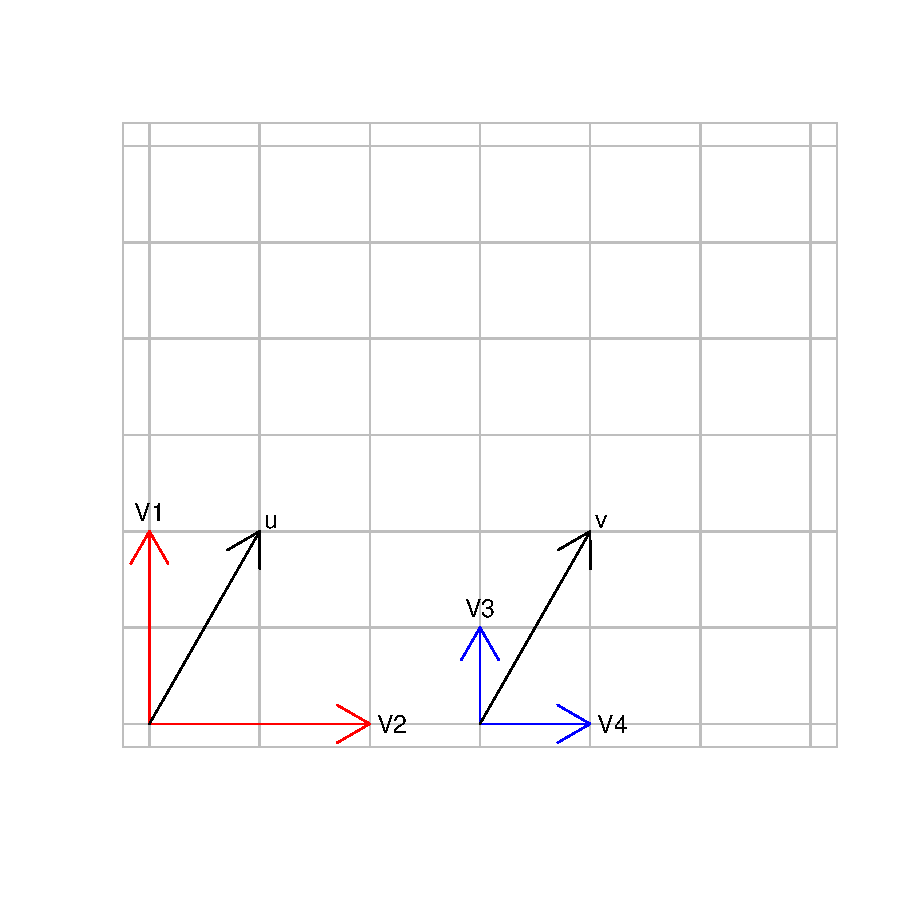
\includegraphics{rapport-graphic}
\newline
Déduction de pourquoi il est impératif de normaliser les données avant 
de travailler avec :\\
Soit $R_{1}$ le référentiel composé par les vecteurs $V_{1}$ et $V_{2}$,
 $R_{2}$ le référentiel composé par les vecteurs $V_{3}$ et $V_{4}$, 
 $\vec{u}$ et $\vec{v}$ deux vecteurs. \\
Si l'on regarde les coordonnées de $\vec{u}$ et $\vec{v}$ exprimée dans 
$R_{1}$, on obtient:
\begin{itemize}
	\item{$\vec{u}=(1,2)$}
	\item{$\vec{v}=(1,2)$}
\end{itemize}
Le produit scalaire de ces deux vecteurs est alors égale à 5.
Si par contre on exprime $\vec{v}$ dans $R_{2}$, ce qui donne $\vec{v}=(2,4)$, et qu'on calcule leur produit scalaire, on obtient 10.
On constate donc que le produit de deux vecteurs ne possédant pas la même norme n'est pas égale au moins dans certains cas.
\paragraph{6.4.}Application des deux méthodes de classification 
(hyperplan médiateur et SVMs) sur le jeu de données "prostate" :
\begin{Schunk}
\begin{Sinput}
> as.vector(t(pred.prostate.mediatorHyperplane <- mediatorHyperplane(prostate)$pred(prostate)))
\end{Sinput}
\end{Schunk}
\begin{Schunk}
\begin{Sinput}
> 
\end{Sinput}
\end{Schunk}
\newline
Discussion des résultats obtenus :

%%%%%%%%%%%%%%%%%%%%%%%%%%%%%%%%%%%%%%%%%%%%%%%%%%%%%%%%%%%%%%%%%%%%%%%%
% SECTION BONUS
%%%%%%%%%%%%%%%%%%%%%%%%%%%%%%%%%%%%%%%%%%%%%%%%%%%%%%%%%%%%%%%%%%%%%%%%
%\newpage
\section{Bonus : algorithme k-NN}
\paragraph{7.1.}Algorithme des \textit{k} plus proches voisins :
\begin{Schunk}
\begin{Sinput}
> 
\end{Sinput}
\end{Schunk}
\paragraph{7.2.}Comparaison de ses performances aux SVMS :
\begin{Schunk}
\begin{Sinput}
> 
\end{Sinput}
\end{Schunk}
\end{document}
